\chapter{Implementation and Evaluation}
\label{chp:chap-five}

\section{Implementation Details}

\subsection{WiFi Controller Implementation}



\subsection{Smart Contract Implementation}



\subsection{Development Framework}

Thanks to the rapid development of blockchain technology, both the private blockchain network deployment tools and DApp\cite{johnston_general_nodate} development framework are state of art. My main contributions are model design, private blockchain network deployment, DApp implementation and system evaluation. The state-of-art developing tools and framework I used are:
\begin{enumerate}
\item Go Ethereum (Geth) is one of the three original implementations (along with C++ and Python) of the Ethereum protocol. It is written in Go, fully open source and licensed under the GNU LGPL v3. And Ethereum is a decentralized platform that runs smart contracts, applications that run exactly as programmed without possibility of downtime, censorship, fraud or third party interference. 
\item Remix, a Solidity IDE used to write, compile and debug Solidity code. Solidity, an object-oriented, high-level language for implementing smart contracts. Smart contracts, detailing in Chapter. 3, are programs which govern the behaviour of accounts within the Ethereum state. 
\item Truffe Suite, consisting of Truffle, Ganache and Drizzle. Trufflle is a world class development environment, testing framework and asset pipeline for blockchains using the Ethereum Virtual Machine (EVM). And Ganache is a personal testing blockchain for Ethereum development. And Drizzle, a collection of front-end libraries, take care of synchronizing contract data, transaction data, etc. 
\end{enumerate}

But still, as the technologies are extensively developing, the implementation of the third-party development tools also keep iterating, which may contain some weird bugs more or less. Here are some challenges while developing the system: 
\begin{enumerate}

\item Proof-of-Authority(PoA) blockchain network is still in the early stages of development. Since the most common consensus algorithm is Proof-of-Work, the current PoA network deployment tools only implement PoA like a adapt version of Proof-of-Work. And so the PoA related code may be buggy.
\item The development tools keep changing, during the developing process, the Drizzle development framework suddenly release a new version and the old version was deprecated. So, the messy dependencies also becomes a challenge.
\end{enumerate}

\section{System Evaluation}

Facing these challenges, I actively involved in the development of open source tools themselves, like report issues, review pull requests and make comments on others' work.

\begin{enumerate}
\item Evaluate the transaction time gap between PoW and PoA consensus algorithm.
\item Evaluate the power consumption difference between PoW and PoA consensus algorithm.
\item Verify the correctness of the result according to the generlized Kelly mechanism.
\end{enumerate}

\subsection{Test Cases and Results}

From test cases and results shown in Fig.\ref{fig:test} and Fig.\ref{fig:result}, we could roughly get the average time for a new user join in the system and re-allocation the bandwidth is around 449.8 ms. The response time is short enough for production.

\begin{figure}[h]
    \centering
    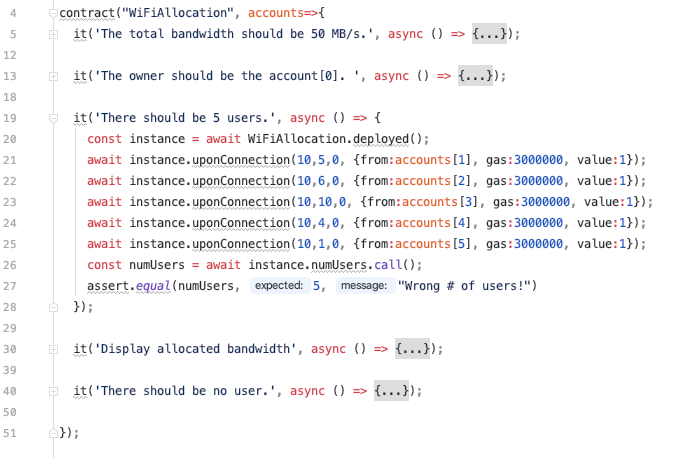
\includegraphics[width=10cm]{My-Thesis/figures/testcases.png}    
    \caption{Test cases}
    \label{fig:test}
\end{figure}

\begin{figure}[h]
    \centering
    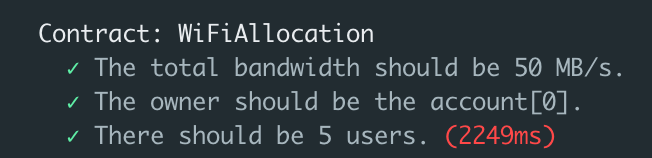
\includegraphics[width=10cm]{My-Thesis/figures/result.png}    
    \caption{Test result}
    \label{fig:result}
\end{figure}

\section{Environment Setup}

The Fig. \ref{fig:environment} shows the experiment environment I used while developing the system. The router is LINKSYS-WRT1900ACS, and the raspberry pi is 4B.

\begin{figure}[h]
    \centering
    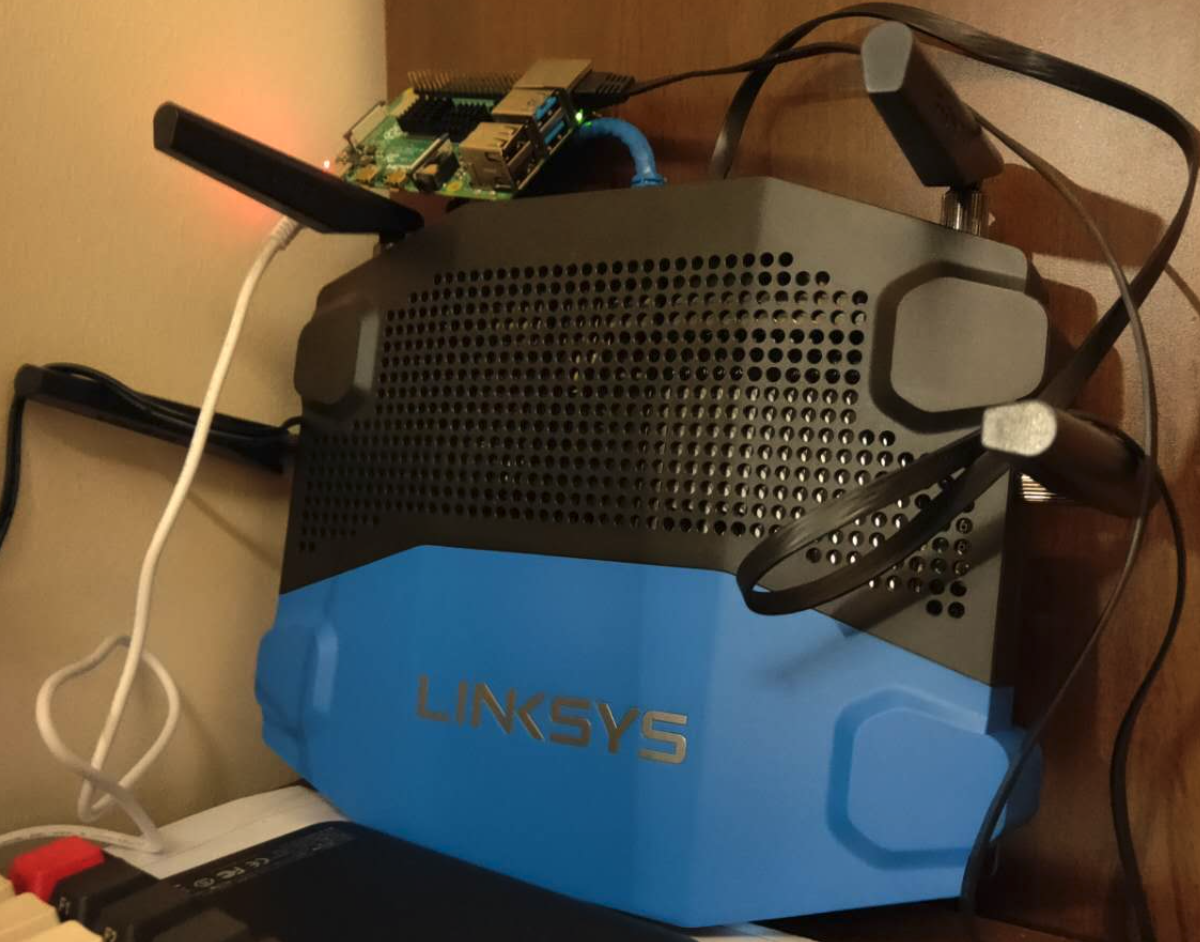
\includegraphics[width=10cm]{My-Thesis/figures/devices.png}    
    \caption{Environment Setup}
    \label{fig:environment}
\end{figure}